\section{Ejercicios 3 y 4 (Round Robin)}
Para testear el algoritmo de Round Robin que permite migración utilizamos los siguientes lotes de tareas:

\textbf{Primer lote:}

\begin{lstlisting}
 # Lote solo con tareas que consumen CPU
 *4 TaskCPU 6
\end{lstlisting}

Sobre el primer lote de tareas hicimos gráficos variando el \textit{quantum} (para 1 y 2 ciclos).
\begin{figure}[h]
 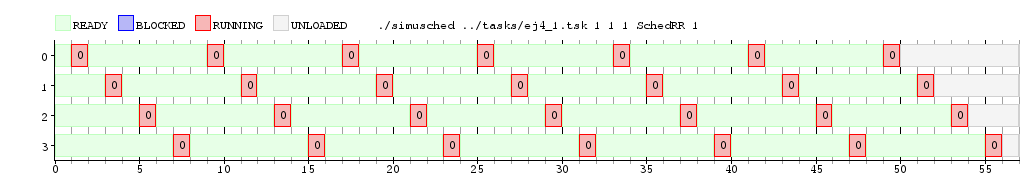
\includegraphics[width=\textwidth]{ej3-4/figs/lote1-quantum1.png}
 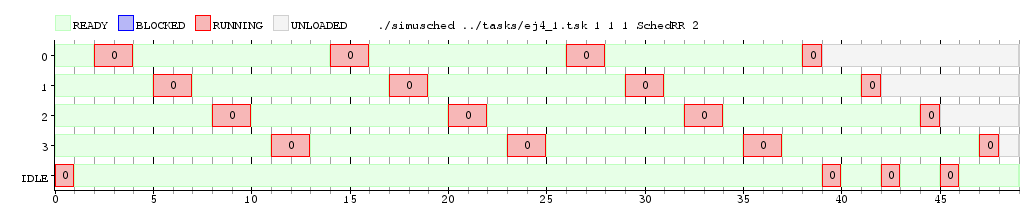
\includegraphics[width=\textwidth]{ej3-4/figs/lote1-quantum2.png}
 \caption{Diagramas de Gantt sobre el primer lote de tareas (para un núcleo, y con quantum igual a 1 y 2, respectivamente).}
 \label{fig:ej4:quantum}
\end{figure}

En la figura~\ref{fig:ej4:quantum} vemos que el algoritmo de Round Robin ejecuta las tareas secuencialmente durante un quantum (que varía de longitud según el caso).

Vemos que sube el tiempo en el que el procesador ejecuta cambios de contexto, porque no se ejecuta una tarea de principio a fin como en el caso anterior.
Al mismo tiempo, mientras más largo es el quantum, menos tiempo se pierde en dichos cambios de contexto (el tiempo de ejecución baja de 56 a 48, incluso con un costo bajo de cambio de contexto).

\textbf{Segundo lote:}
El segundo lote contiene también tareas con bloqueos.

\begin{lstlisting}
 # Tareas que se bloquean y que comen CPU
 *2 TaskConsola 5 1 10
 @3
 *2 TaskCPU 15
\end{lstlisting}

En estos casos el algoritmo de Round Robin tiene la ventaja adicional de que (como vemos en la figura~\ref{fig:ej4:cores}), ante un bloqueo, el procesador cambia de proceso y aprovecha el tiempo de CPU.
\begin{figure}[h]
 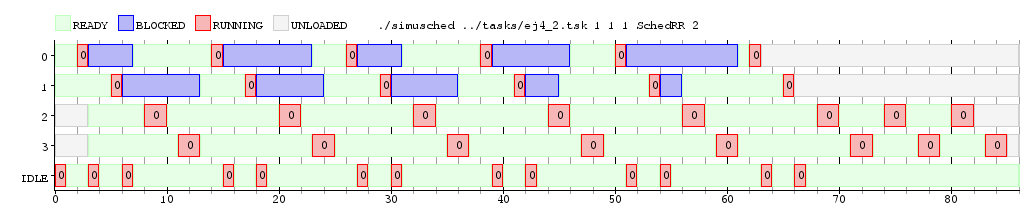
\includegraphics[width=\textwidth]{ej3-4/figs/lote2-1core.png}
 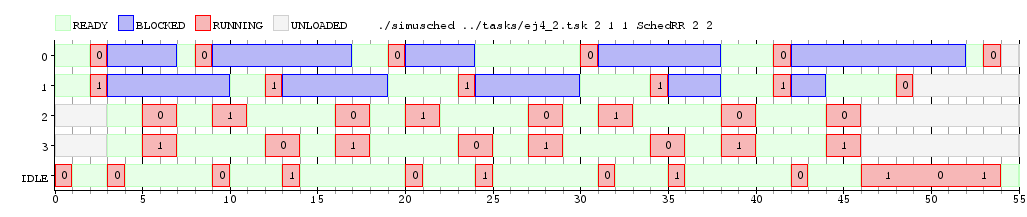
\includegraphics[width=\textwidth]{ej3-4/figs/lote2-2core.png}
 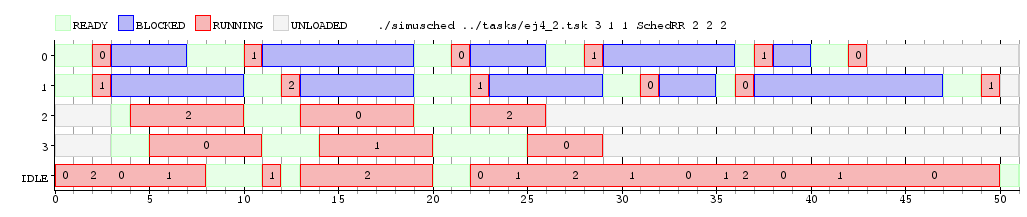
\includegraphics[width=\textwidth]{ej3-4/figs/lote2-3core.png}
 \caption{Diagramas de Gantt sobre el segundo lote de tareas (para 1, 2 y 3 núcleos, fijando el quantum en 2).}
 \label{fig:ej4:cores}
\end{figure}

En el caso de un núcleo no se nota tanto la mejora porque todos los bloqueos terminan antes de que el ciclo vuelva al mismo proceso, pero ya en 2 núcleos vemos que el algoritmo, en el tick 9, asigna la tarea 2 (en vez de la 1) al procesador 1, porque el otro no estaba disponible.
Este comportamiento se repite a lo largo del resto de la ejecución. En el caso de 3 núcleos, incluso, el mismo proceso puede ejecutar durante varios quantums seguidos a pesar de que sean más la cantidad de tareas que la de procesadores.

